\chapter{Aplicación web}\label{cap:diseno}

Este capítulo reúne todo lo que corresponde al producto: qué debe hacer, cómo se diseñó, cómo
se construyó y dónde se despliega. Recorre, en un único hilo, los requisitos que fijan el
alcance, la arquitectura y el modelo de datos que le dan forma, la implementación que los
materializa y la topología pública en la que se sirve, de modo que el lector no tenga que
saltar entre capítulos para reconstruir una sola pieza del sistema. El Capítulo~\ref{cap:nucleo-investigacion}
recoge, por separado, el otro núcleo del trabajo: los algoritmos de recomendación y su
evaluación, que se apoyan en esta misma plataforma pero se estudian con su propio rigor
experimental.

\section{Análisis de requisitos}\label{cap:requisitos}

El sistema distingue tres actores con acceso real. El visitante, sin autenticar, puede
consultar el catálogo, la ficha de cada juego con su procedencia, un perfil público y la
recomendación por popularidad. La persona usuaria, titular de una cuenta controlada, gestiona
además su propia lista de pendientes, valora juegos e inventaría sus copias físicas y
digitales. La cuenta simulada es una variante etiquetada con claridad como tal, precargada
para que el tribunal y cualquier visitante puedan recorrer el sistema sin crear una cuenta
propia. Dos actores adicionales, un perfil de administración de cuentas y catálogo y un perfil
de personal investigador con acceso al panel de comparación de algoritmos, se incluyen en el
análisis para dar contexto completo al modelo, aunque su implementación queda fuera del
alcance descrito en esta memoria.

El modelo de dominio distingue tres áreas: catálogo, biblioteca personal y cuentas. En el
catálogo, la entidad central es la obra (\texttt{GameWork}), la identidad canónica de un
título de videojuego con independencia de la plataforma y de la edición concreta, con un
identificador único universal (UUID) generado en el momento de la importación, de modo que
cambiar de proveedor de enriquecimiento, o prescindir de él, nunca obliga a renumerar el
catálogo. Cada obra puede tener varias publicaciones, una por plataforma; cada publicación
puede tener a su vez varias ediciones. La obra guarda también, de forma deliberadamente
desnormalizada, la fecha de primer lanzamiento y la valoración agregada de origen, para que
filtrar por año o por nota sea un recorrido de índice y no una agregación sobre cientos de
miles de publicaciones en cada consulta, y los alias bilingües sostienen la búsqueda tolerante
a errores tipográficos mediante un índice de trigramas. La procedencia de cada obra (fuente,
identificador de origen, licencia, fecha de recuperación y huella del contenido) se conserva
junto a ella, no como un metadato aparte que se pueda perder. En la biblioteca personal, la
entrada de biblioteca representa la relación entre una persona y una obra: su estado en la
lista de pendientes y su valoración, esta última almacenada como un entero de medias estrellas
entre uno y diez, nunca como un número en coma flotante que introduciría precisión falsa, con
una restricción de unicidad que impide más de una entrada por persona y obra. El historial de
cambios de estado se conserva como un registro de solo anexado, de forma que se puede
reconstruir cuándo una persona empezó, dejó o retomó un juego, y las copias en propiedad
representan cada ejemplar físico o digital, con su formato, su publicación y su edición, y una
clave de idempotencia que evita duplicados cuando el usuario reintenta un alta que en realidad
ya se había registrado. En cuentas, el sistema usa el modelo de usuario de Django directamente
y añade sobre él las entidades necesarias para identificar de forma inequívoca qué cuentas son
simuladas, con una restricción de base de datos que impide, incluso por error de aplicación,
que una cuenta simulada deje de estar marcada como tal.

De los noventa y cuatro requisitos identificados en el análisis, noventa y dos están
completos, con evidencia verificable en \texttt{docs/verification/} o en las firmas de
aceptación por fase. Entre los completos están la autenticación con cuentas simuladas, la
búsqueda y el filtrado del catálogo, la ficha de detalle con su procedencia, el ciclo completo
de biblioteca y copias, la portabilidad de la colección (exportación versionada y una
importación validada con previsualización, errores fila a fila y reglas deterministas de
conflicto), la privacidad de perfil y, como desarrolla en profundidad el
Capítulo~\ref{cap:nucleo-investigacion} de esta memoria, las tres familias completas de
recomendación con su protocolo de evaluación offline, incluidas sus métricas de precisión,
cobertura, diversidad y novedad por cohorte de usuario. Los dos requisitos que quedan
pendientes son parciales, no partidas sin empezar, y ambos pertenecen al mismo contrato de
evaluación: repetir la comparación de algoritmos con varias semillas, más allá de la ejecución
única ya publicada como v15, y retroproyectar sobre esa misma ejecución histórica la captura de
entorno y consumo de recursos que el ejecutor paralelo ya sabe registrar para comparaciones
futuras. Ambos quedan documentados como líneas de continuación explícitas en el
Capítulo~\ref{cap:conclusiones}, no presentados como si ya existieran.

Los requisitos no funcionales se agrupan en cinco familias. La reproducibilidad exige que el
sistema arranque de forma determinista en un entorno local documentado, con todas las
dependencias fijadas a una versión exacta. La legalidad y procedencia de datos exige que cada
dato del catálogo conserve su fuente, su licencia y su fecha de recuperación, con la elección
de cada fuente documentada junto con sus términos de uso. La accesibilidad y el diseño
responsive exigen que los flujos principales funcionen con teclado y en anchuras de
escritorio y de móvil, verificables frente a las Pautas de Accesibilidad para el Contenido Web
(WCAG) 2.2 en nivel AA~\cite{wcag22}. La seguridad de la demostración controlada exige que
ningún secreto aparezca en el control de versiones, en los paquetes servidos al navegador ni
en ningún artefacto público, y que toda acción de escritura quede protegida contra
falsificación de petición en sitios cruzados. La calidad visual de producto, por último, exige
que la interfaz presente la densidad, la tipografía y el tratamiento de imagen propios de un
producto de catalogación cuidado, no de un prototipo funcional sin pulir.

Algunas reglas de negocio gobiernan el comportamiento del sistema con independencia de la
pantalla desde la que se disparen. La identidad de una obra es siempre un identificador
interno propio: el identificador del proveedor externo se guarda solo como procedencia, nunca
como clave. El contenido descargable y las expansiones se muestran dentro de la página de su
obra padre, nunca como resultado independiente del catálogo. Los detalles privados de
propiedad, como notas o datos de compra, no aparecen en ninguna proyección pública bajo
ninguna circunstancia. La valoración se almacena siempre como un entero de medias estrellas.
La recomendación por popularidad se calcula solo sobre actividad de cuentas simuladas y nunca
se presenta como personalizada, mientras que la recomendación basada en la actividad propia de
una persona nunca cae de forma silenciosa al baseline de popularidad cuando no hay suficiente
historial: muestra en su lugar un estado explícito de bienvenida. Registrar de nuevo una copia
con la misma clave de idempotencia devuelve la copia existente en lugar de crear un duplicado.
El acceso a fuentes de datos externas, por último, queda siempre confinado a comandos de
gestión fuera de línea: ninguna petición de un visitante o de una persona usuaria dispara,
directa o indirectamente, una llamada a un proveedor externo.

La Tabla~\ref{tab:trazabilidad-familias} recorre las diecisiete familias de requisitos del
proyecto, con cuántos de cada una están completos y verificados frente a los que quedan
pendientes. Cada fila es, en sí misma, una entrada de trazabilidad: el código de familia enlaza
directamente con los identificadores individuales de \texttt{.planning/REQUIREMENTS.md}; el
estado de cada uno de ellos remite a su vez a una firma de aceptación por fase o a un plan
concreto en \texttt{docs/verification/}.

\begin{table}[H]
\centering
\caption{Trazabilidad de requisitos de SavePoint, por familia.}\label{tab:trazabilidad-familias}
\tablecompact
\begin{tabularx}{\textwidth}{@{}>{\ttfamily\raggedright\arraybackslash}p{0.14\textwidth}Yrr@{}}
\textnormal{Familia} & \textnormal{Cubre} & \textnormal{Completos} & \textnormal{Total} \\
\hline
AUTH & Autenticación y sesión & 2 & 2 \\
PROF & Perfil personal y público & 4 & 4 \\
CAT & Catálogo, búsqueda y filtrado & 6 & 6 \\
LIB & Biblioteca y valoración & 4 & 4 \\
INV & Inventario de copias & 5 & 5 \\
DATA & Procedencia y gobierno de datos & 8 & 8 \\
REC & Algoritmos de recomendación & 10 & 10 \\
EVAL & Protocolo y laboratorio de evaluación & 12 & 14 \\
SEC & Seguridad & 8 & 8 \\
OPS & Operaciones y copia de seguridad & 5 & 5 \\
QUAL & Calidad de producto y accesibilidad & 5 & 5 \\
DOC & Documentación y registro & 6 & 6 \\
AGENT & Metodología de ingeniería & 6 & 6 \\
PORT & Portabilidad de datos & 4 & 4 \\
PRIV & Privacidad & 2 & 2 \\
SOCIAL & Relaciones sociales & 3 & 3 \\
ADMIN & Administración & 2 & 2 \\
\hline
\textbf{Total} & & \textbf{92} & \textbf{94} \\
\end{tabularx}
\end{table}

Una única familia conserva requisitos pendientes, \texttt{EVAL}, y los dos que quedan son la
repetición con varias semillas y la captura retroactiva de entorno ya descritas; ningún
requisito completo depende de uno pendiente para su propia verificación, de modo que ese
trabajo futuro no invalida ninguna evidencia ya cerrada.

\section{Diseño de la arquitectura}\label{sec:web-diseno}

SavePoint es un monolito modular con dos ejecutables. El backend, en \texttt{apps/api/}, usa
Django~\cite{django} con soporte a largo plazo y Django REST Framework (DRF)~\cite{drf} sobre
PostgreSQL~\cite{postgresql}, con el mapeo objeto-relacional (ORM) de Django como interfaz de
persistencia; sus módulos se separan por dominio (\texttt{catalogue}, \texttt{library},
\texttt{accounts}, \texttt{recommendations}, \texttt{evaluation}, \texttt{social},
\texttt{audit}), pero comparten despliegue y base de datos. El frontend, en
\texttt{apps/web/}, es una aplicación Next.js~\cite{nextjs} con React~\cite{react} y
TypeScript en modo estricto, que renderiza en el servidor las páginas públicas; el navegador
solo llama a rutas del mismo origen de Next.js, que las reescribe hacia el backend. Los
trabajos de recomendación y evaluación se
ejecutan como comandos fuera de la petición HTTP: la aplicación publica sus resultados, pero no
vuelve a calcular la evidencia científica en el navegador. La Figura~\ref{fig:arquitectura}
representa esta arquitectura por capas, y el registro de decisión ADR-001 recoge el contexto
completo de esta elección.

Esa elección no fue automática. El dominio de SavePoint (obras, ediciones, copias,
valoraciones, biblioteca) es relacional y con mucha escritura estructurada, el tipo de
problema para el que Django y su ORM están pensados desde el principio, con autenticación,
panel de administración, migraciones y validación ya resueltos en el propio marco de trabajo.
Frente a alternativas más ligeras como FastAPI con SQLAlchemy, que habrían obligado a componer
esas mismas piezas a mano, Django ofrece esa base madura sin coste adicional. Frente a servir
la interfaz con plantillas de Django y HTMX, que habría evitado duplicar el contrato de datos
entre backend y frontend, se prefirió un frontend Next.js separado porque el panel
experimental de recomendación necesitaba una interfaz más rica de lo que las plantillas del
lado del servidor ofrecen con comodidad, sin perder por ello el renderizado en servidor que la
accesibilidad y el primer pintado rápido piden. Una arquitectura de microservicios, por
último, se descartó por su coste operativo y de trazabilidad en un proyecto de un único
desarrollador: separar servicios solo se justifica cuando hay una necesidad medida que lo
pida, no por anticipado.

PostgreSQL es la única base de datos de aplicación y de pruebas de integración, en desarrollo,
en pruebas y en despliegue, sin sustituir nunca por una base más ligera en ningún entorno. El
registro ADR-002 explica por qué: el modelo de datos de SavePoint depende de restricciones de
unicidad, de transacciones y de búsqueda por similitud de texto que SQLite soporta de forma
incompleta y que una base documental como MongoDB no ofrece con la misma garantía de
integridad relacional. Usar SQLite en local y PostgreSQL en producción, la solución más
barata a corto plazo, se descartó explícitamente porque introduce una asimetría entre entornos
que un banco de pruebas reproducible no se puede permitir: una consulta que funciona en SQLite
y falla en PostgreSQL, o viceversa, sería un defecto del propio diseño experimental, no del
código. Todo el sistema se levanta, en consecuencia, con Docker Compose a partir de los tres
componentes de aplicación (base de datos, API y frontend), cada uno construido desde su propio
fichero de Docker con versiones de dependencias fijadas; junto a ellos, Compose orquesta además
un contenedor de \textit{worker} independiente por cada variante de algoritmo de recomendación
publicada, de modo que la ejecución completa del entorno reproducible levanta más de una decena
de contenedores adicionales de cómputo, no solo los tres de aplicación. Un trabajo cuyo objeto
de estudio es la reproducibilidad de una comparación de algoritmos necesita, antes que nada,
que el propio entorno de ejecución sea reproducible, y los contenedores eliminan esa variable
en cualquier máquina que lo levante.

Para la demostración pública se adoptó una topología repartida entre tres proveedores
gratuitos en lugar de un único servicio con predespliegue de contenedores, por una restricción
de partida no negociable: coste cero, sin tarjeta de pago ni recursos de facturación
habilitados. Vercel construye de forma nativa el frontend Next.js y reescribe del lado del
servidor las llamadas a la API hacia Render, que construye y sirve la imagen del backend, y
Neon suministra PostgreSQL como servicio gestionado a Render; los tres se eligieron porque cada
uno ofrece, en su nivel gratuito, la primitiva concreta que SavePoint necesita sin exigir una
tarjeta para activarse, una combinación que ningún proveedor único cubre por sí solo. La
Sección~\ref{cap:despliegue}, más adelante en este mismo capítulo, desarrolla esta topología,
sus límites conocidos y el estado actual del despliegue; el registro ADR-005 recoge la
decisión completa.

Cada decisión de diseño con consecuencias materiales queda registrada como registro de
decisión de arquitectura (ADR), con un formato fijo de contexto, alternativas, decisión,
evidencia, consecuencias y reversibilidad. La Tabla~\ref{tab:adr-resumen} resume el conjunto
vigente; los capítulos correspondientes citan cada registro donde es relevante.

\begin{table}[H]
\centering
\begin{tabularx}{\textwidth}{ | Y | Z | }
    \hline
    \textbf{Registro} & \textbf{Decisión} \\
    \hline
    ADR-001 & Monolito modular Django/DRF con frontend Next.js separado. \\
    \hline
    ADR-002 & PostgreSQL como única base de datos de aplicación y de pruebas. \\
    \hline
    ADR-003 & Corpus curado inicial de Wikidata, bajo dominio público, con revisión de licencia por archivo de Commons. \\
    \hline
    ADR-004 & Sesión de Django y frontera de mismo origen entre frontend y backend. \\
    \hline
    ADR-005 & Despliegue público de coste cero repartido entre Vercel, Render y Neon. \\
    \hline
    ADR-006 & IGDB como fuente del catálogo a escala real, con portadas servidas por enlace directo. \\
    \hline
    ADR-007 & Heurístico determinista de afinidad por géneros como recomendador inicial explicable. \\
    \hline
    ADR-008 & Ratings externos gobernados por snapshot versionado, con enriquecimiento acotado desde RAWG. \\
    \hline
    ADR-009 & Familias de algoritmos de recomendación y su ejecución como \textit{workers} aislados. \\
    \hline
\end{tabularx}
\caption{Registros de decisión de arquitectura vigentes.}
\label{tab:adr-resumen}
\end{table}

La Figura~\ref{fig:modelo-dominio} representa el modelo de dominio completo, agrupado por
catálogo, biblioteca personal, cuentas e investigación. El diseño de datos separa obra,
edición, plataforma y copia, y distingue en todo momento la proyección pública de los datos
privados de cada persona; las restricciones de integridad, como la unicidad de una entrada de
biblioteca por persona y obra o el rango válido de una valoración, viven en la propia base de
datos y no solo en la capa de aplicación, para que ningún cliente pueda saltárselas escribiendo
directamente contra la API. Los snapshots y artefactos que alimentan el laboratorio de
recomendación incorporan versión y huella criptográfica, de forma coherente con la exigencia
de reproducibilidad que recorre todo el diseño.

\section{Implementación y verificación}\label{cap:implementacion}

El backend se divide en los módulos de cuentas, catálogo, biblioteca, social, recomendaciones,
evaluación y auditoría, descritos en su reparto de dominio en la sección anterior. El frontend
implementa
las vistas de catálogo, detalle, colección, perfil, listas, comentarios, recomendaciones y
panel de investigación. La importación y el gobierno de datos se ejecutan como procesos
explícitos fuera de la petición HTTP; las recomendaciones se publican mediante snapshots y los
experimentos se ejecutan mediante comandos offline. La Tabla~\ref{tab:stack-resumen} recoge
las versiones principales del entorno reproducible que Docker Compose orquesta.

\begin{table}[H]
\centering
\begin{tabularx}{\textwidth}{ | Y | Y | Y | }
    \hline
    \textbf{Componente} & \textbf{Versión} & \textbf{Papel} \\
    \hline
    Django + Django REST Framework & 5.2 LTS / 3.18 & Dominio, autenticación, ORM, sesiones y API. \\
    \hline
    PostgreSQL & 18.6 & Base de datos de aplicación y de pruebas de integración. \\
    \hline
    Next.js + React & 16.3 / 19.2 & Renderizado en servidor, rutas y componentes. \\
    \hline
    TypeScript & 6.0, modo estricto & Tipado del frontend. \\
    \hline
\end{tabularx}
\caption{Versiones principales del entorno reproducible. El Apéndice~\ref{ap:implementacion-detallada} recoge la tabla completa.}
\label{tab:stack-resumen}
\end{table}

Toda tarea de datos a escala es un comando de gestión de Django, ejecutable fuera de la
petición HTTP e idempotente: el importador de IGDB recorre la API por lotes con un cursor de
identificador reanudable que un disparador de base de datos impide retroceder, de modo que una
ejecución interrumpida siempre reanuda hacia delante desde el progreso real; el comando de
gobierno del corpus aplica la lista de plataformas permitidas y calcula las razones de
exclusión sin enumerar todo el catálogo en el proceso; y la cadena de arranque del despliegue
encadena migración, importación, creación de cuentas y semilla antes de ceder el control al
servidor, deteniéndose ante el primer paso fallido para que el chequeo de salud nunca se ponga
en verde con una inicialización parcial. La búsqueda del catálogo es tolerante a errores
tipográficos: primero intenta coincidencia exacta, después por prefijo y por último por
similitud de trigramas, siempre sobre el índice de alias normalizados y sin ninguna llamada
externa. La página de recomendaciones por afinidad de géneros, descrita como recomendador
inicial explicable en el Capítulo~\ref{cap:nucleo-investigacion}, se calcula en tiempo de
petición a partir de la biblioteca de la persona autenticada, sin paso de entrenamiento ni
almacén de características persistido; cada respuesta lleva una huella criptográfica de su
entrada y de su resultado, de modo que dos llamadas idénticas producen exactamente la misma
salida.

En el frontend, el navegador solo llama a rutas del mismo origen de Next.js, que las reescribe
del lado del servidor hacia el backend con el destino tomado de una variable de entorno visible
únicamente en el servidor; así, las cookies de sesión y de protección contra falsificación de
petición en sitios cruzados que emite Django siguen siendo del mismo origen, sin necesidad de
compartir recursos entre orígenes con credenciales. La interfaz está disponible en español y en
inglés mediante diccionarios por idioma, con una prueba de paridad que falla si una clave existe
en un idioma pero no en el otro. El Apéndice~\ref{ap:implementacion-detallada} desarrolla estos
mecanismos con extractos de código referenciados. La Figura~\ref{fig:inicio} documenta la
portada de la demostración y la Figura~\ref{fig:recomendaciones-ui} muestra la vista de
recomendaciones disponible en el proyecto; son capturas de interfaz, no evidencia de calidad
de ranking ni de resultados experimentales.

\begin{figure}[H]
\centering
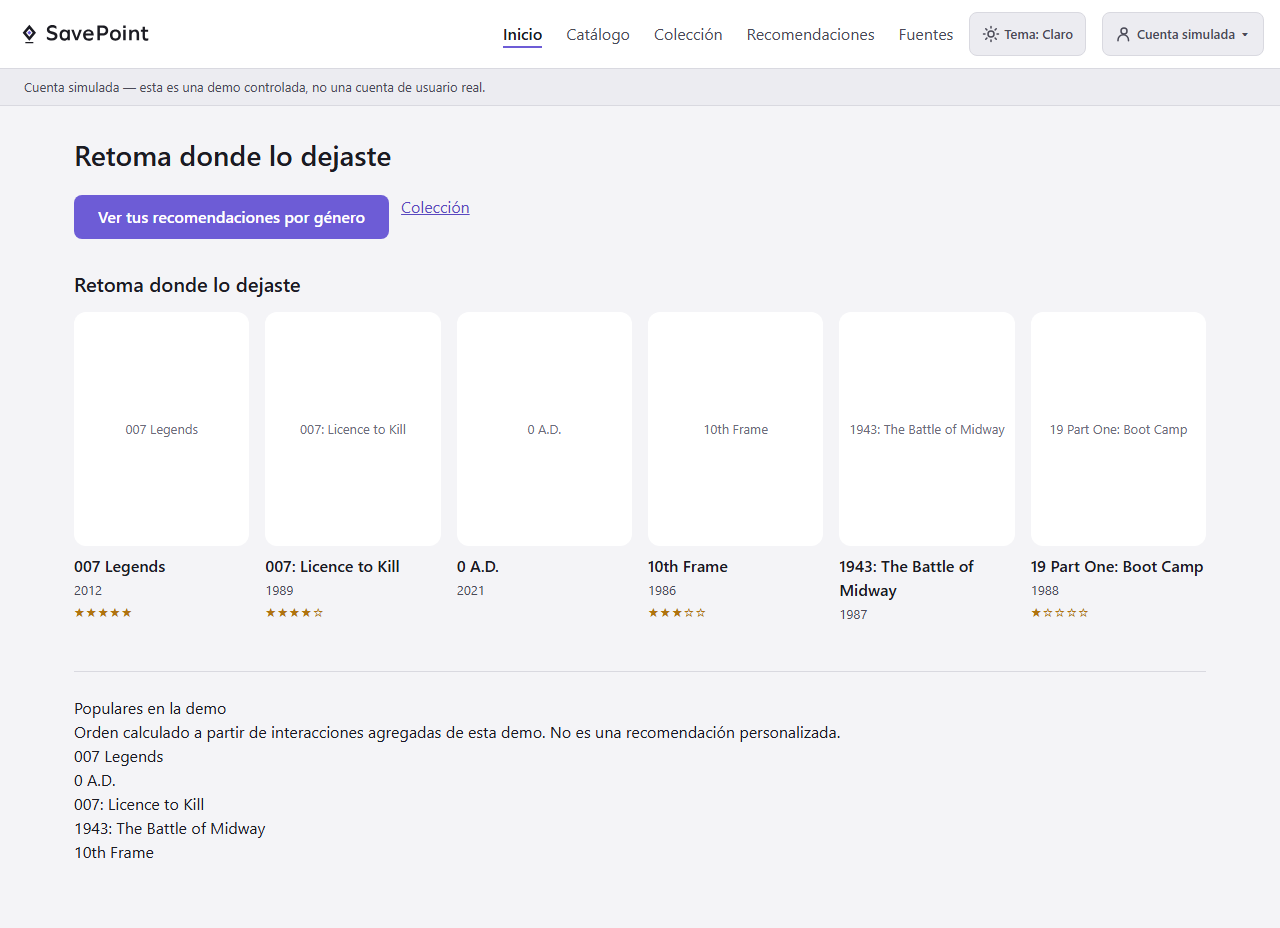
\includegraphics[width=0.82\textwidth]{figures/captura-home-claro}
\caption{Portada de SavePoint en tema claro. Fuente: captura del proyecto.}\label{fig:inicio}
\end{figure}

\begin{figure}[H]
\centering
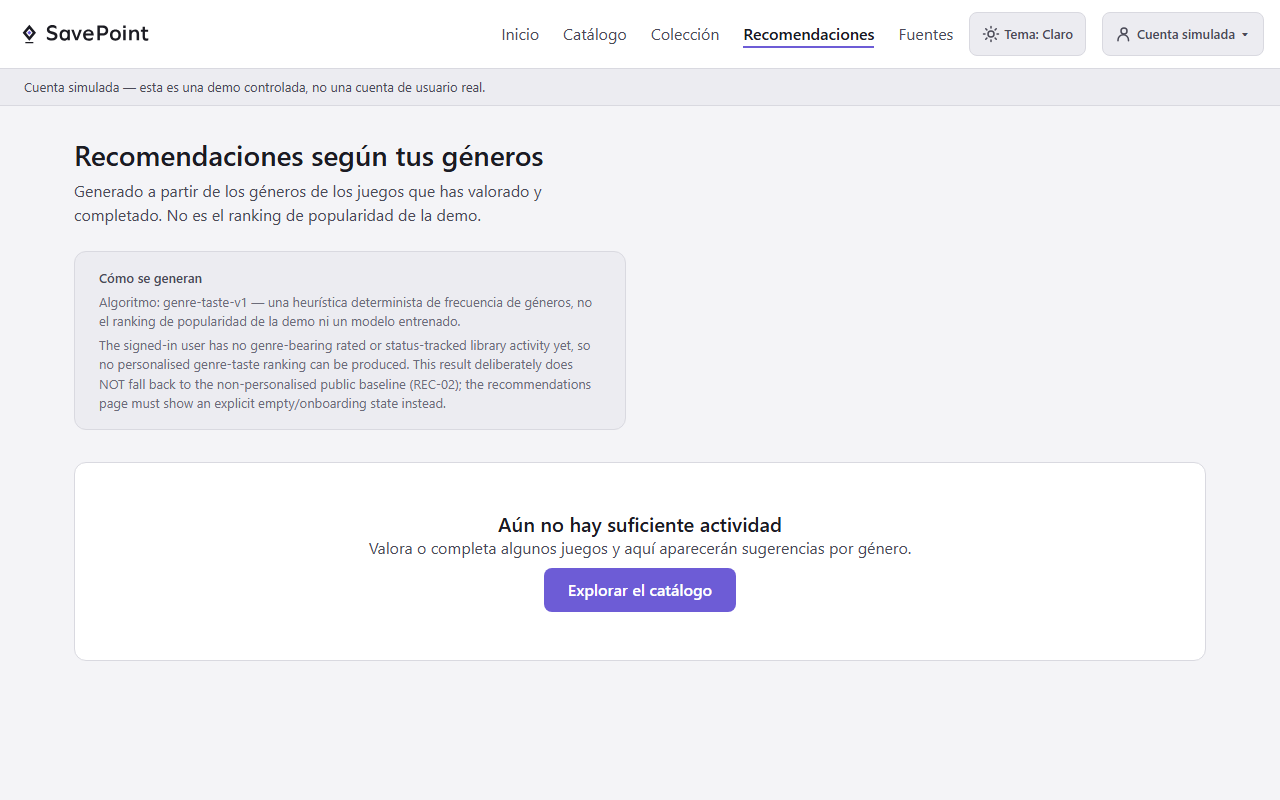
\includegraphics[width=0.82\textwidth]{figures/captura-recomendaciones}
\caption{Vista de recomendaciones de la aplicación. Fuente: captura del proyecto.}\label{fig:recomendaciones-ui}
\end{figure}

La verificación combina pruebas de backend contra PostgreSQL real (unitarias e integración en
una única suite \texttt{pytest}, sin separarlas en conteos independientes), pruebas de
frontend con Vitest y un recorrido de navegador con Playwright que integra los casos de
accesibilidad mediante \texttt{axe}, sin un conteo aislado solo de accesibilidad. El cierre de
evidencia de la Fase 7, ejecutado el 14 de septiembre de 2026 y registrado en
\texttt{docs/verification/phase-07-launch-gate.md} y en \texttt{07-VERIFICATION.md}, deja como
última regresión completa 736 pruebas de backend, 70 de frontend y 56 de navegador, las tres
en verde y sin omitidas. Las evidencias de seguridad, migraciones, privacidad, importación y
exportación se citan desde \texttt{docs/verification/}.

\section{Despliegue}\label{cap:despliegue}

La restricción de partida del despliegue público es la misma que ya fijó su diseño: coste
cero, sin introducir ninguna tarjeta de pago ni habilitar ningún recurso de facturación. La
Tabla~\ref{tab:topologia} recoge el contrato de cada superficie.

\begin{table}[H]
\centering
\begin{tabularx}{\textwidth}{ | Y | Y | Y | }
    \hline
    \textbf{Superficie} & \textbf{Servicio} & \textbf{Contrato} \\
    \hline
    Interfaz de navegador & Vercel Hobby & Construye el frontend Next.js; reenvía del lado del servidor las rutas de la API y de salud hacia Render. \\
    \hline
    API & Render Free & Construye la imagen de la API con el catálogo local congelado y expone la ruta de salud. \\
    \hline
    Base de datos & Neon Free & Proyecto \texttt{autumn-breeze-06234770}, rama \texttt{production}; suministra PostgreSQL a Render. \\
    \hline
\end{tabularx}
\caption{Topología pública aprobada, de coste cero.}
\label{tab:topologia}
\end{table}

El navegador solo ve el origen HTTPS de Vercel. La variable que apunta al backend existe
únicamente en el entorno de servidor de Next.js, de modo que las cookies de sesión y de
protección contra falsificación de petición en sitios cruzados que emite Django siguen siendo
del mismo origen. En Render, la cadena de arranque encadena migración, importación del
catálogo, creación de cuentas simuladas y semilla; solo entonces cede el control al servidor
\texttt{gunicorn}, con cada paso idempotente y protegido con un bloqueo consultivo, de modo que
un paso fallido detiene el arranque, tal como resume la Figura~\ref{fig:despliegue-flujo}.

\begin{figure}[H]
    \centering
    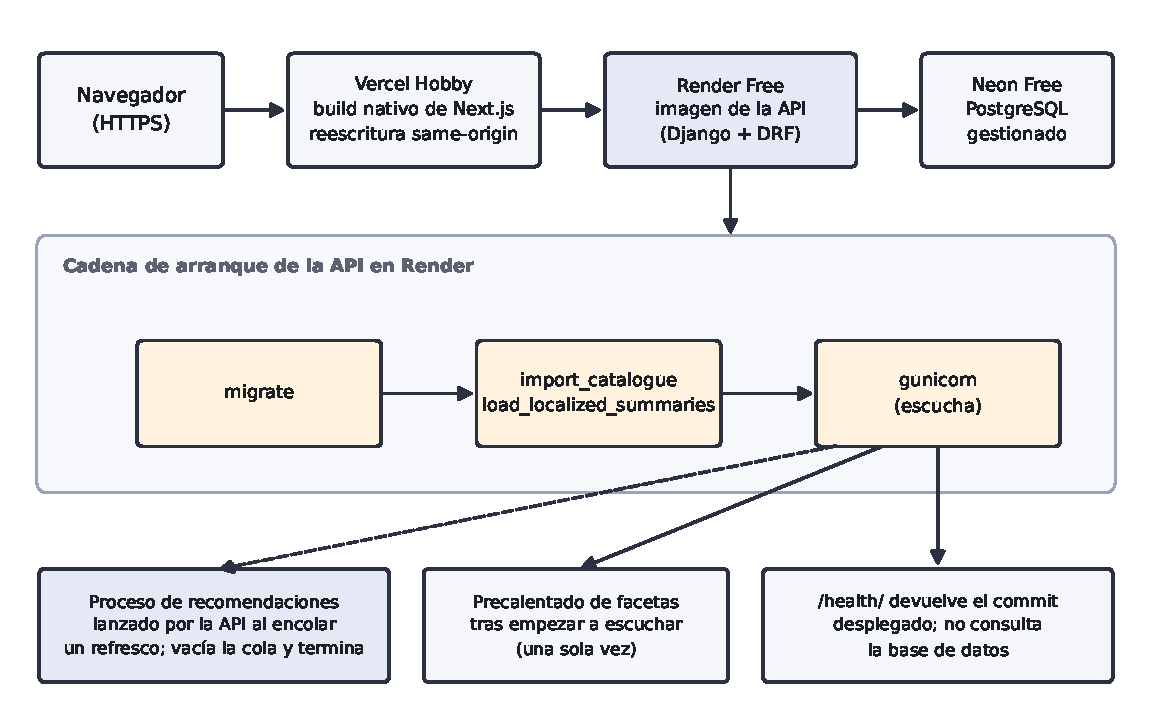
\includegraphics[width=0.92\textwidth]{figures/despliegue-flujo.pdf}
    \caption{Topología de despliegue público y cadena de arranque en Render.}
    \label{fig:despliegue-flujo}
\end{figure}

Docker Compose sigue siendo el entorno reproducible canónico, con los tres componentes de
aplicación (base de datos, API y frontend) y los \textit{workers} de recomendación construidos
desde sus ficheros de Docker. La equivalencia con el
despliegue público es funcional, de versiones, de commit y de datos, no de imagen byte a
byte: el frontend público lo construye Vercel de forma nativa y no ejecuta la imagen de Docker
del frontend, una diferencia de despliegue documentada, no una divergencia de comportamiento.
Si cualquier servicio gratuito duerme, cambia sus términos o desaparece, el entorno local sigue
disponible sin conexión. Los límites conocidos del nivel gratuito se declaran de forma
explícita: el servicio de la API en Render duerme tras quince minutos sin tráfico, de modo que
un visitante puede encontrar un arranque en frío de cerca de un minuto; las cuotas mensuales de
los tres proveedores pueden suspender un servicio, y el nivel gratuito no promete copias de
seguridad ni restauración.

La demostración pública está en vivo desde el 5 de septiembre de 2026, con la prueba de humo en
verde contra la revisión desplegada. En ese despliegue sirve la interfaz anterior al rediseño
contra el corpus curado de ciento cincuenta juegos de Wikidata: el rediseño de la interfaz y el
catálogo a escala real no están en el despliegue público, sino integrados en la rama principal
y ejecutados en el entorno local de Docker Compose. El frontend rediseñado llegó a construirse
en Vercel, pero la base de datos desplegada todavía contiene solo el corpus curado, de modo que
la vista de catálogo da error contra ese despliegue; se revisó esta situación y se decidió
dejar el despliegue público actual como está por ahora, con la demostración ante el tribunal
ejecutándose desde el entorno local reproducible. Conectar el despliegue a datos reales de
internet (cargar el catálogo de IGDB en una base de datos desplegada, aplicar las migraciones
nuevas y ajustar la configuración de hosts y de proxies) queda pospuesto al final del proyecto:
es una decisión registrada, no un defecto pendiente.

Este capítulo ha descrito el producto completo, de los requisitos al despliegue. El
Capítulo~\ref{cap:nucleo-investigacion} recorre el otro núcleo del trabajo, los algoritmos de
recomendación que se construyen sobre esta misma plataforma, y el Capítulo~\ref{cap:conclusiones}
cierra la memoria con el grado de cumplimiento de los objetivos y las líneas de continuación.
